%Metroplolis Beamer Theme: https://github.com/matze/mtheme
\documentclass[aspectratio=169, 10pt, dvipsnames, handout]{beamer}
\usetheme{metropolis}
\usepackage{appendixnumberbeamer, lmodern, bookmark, kbordermatrix,fontawesome}
\usepackage{booktabs}
% \usepackage[sorting=none]{biblatex}
\usepackage[scale=2]{ccicons}
\usepackage{pgfplots}
\usepgfplotslibrary{dateplot}
\usepackage{xspace}
\newcommand{\themename}{\textbf{\textsc{metropolis}}\xspace}
\usepackage{bbm}
\usepackage{tikz, graphicx}
\usepackage{caption, subcaption}
\usepackage{multicol}
% \usepackage[dvipsnames]{xcolor}
\usepackage{animate}
\usepackage{scalerel,xparse}
\usepackage[style=british]{csquotes}

\title{GNNMetrics, a package for optimizing and understanding MMD
parametrization for evaluating generative GNNs on protein datasets.}
% \subtitle{Lab Update}
\date{\today}
\author{Philip Hartout}

% \titlegraphic{\hfill\includegraphics[height=1.5cm]{logo.pdf}}

\hypersetup{
  colorlinks=true,
  linkcolor=orange,
  filecolor=orange,
  urlcolor=orange,
}

\def\signed #1{{\leavevmode\unskip\nobreak\hfil\penalty50\hskip1em
  \hbox{}\nobreak\hfill #1%
  \parfillskip=0pt \finalhyphendemerits=0 \endgraf}}

\newsavebox\mybox
\newenvironment{aquote}[1]
  {\savebox\mybox{#1}\begin{quote}\openautoquote\hspace*{-.7ex}}
  {\unskip\closeautoquote\vspace*{1mm}\signed{\usebox\mybox}\end{quote}}

\titlegraphic{%
  
\includegraphics[width=.2\textwidth]{figures/mlcb-transparent.png}\hfill
  
\includegraphics[width=.2\textwidth]{figures/dbsse-transparent.png}\hfill
  
\includegraphics[width=.2\textwidth]{figures/eth-transparent.png}
}

\makeatletter
\setbeamertemplate{title page}{
  \begin{minipage}[b][\paperheight]{\textwidth}
    \vfill%
    \ifx\inserttitle\@empty\else\usebeamertemplate*{title}\fi
    \ifx\insertsubtitle\@empty\else\usebeamertemplate*{subtitle}\fi
    \usebeamertemplate*{title separator}
    \ifx\beamer@shortauthor\@empty\else\usebeamertemplate*{author}\fi
    \ifx\insertdate\@empty\else\usebeamertemplate*{date}\fi
    \ifx\insertinstitute\@empty\else\usebeamertemplate*{institute}\fi
    \vfill
    \ifx\inserttitlegraphic\@empty\else\inserttitlegraphic\fi
    \vspace*{1cm}
  \end{minipage}
}
\makeatother

\usetikzlibrary{shapes.geometric, arrows}

\tikzstyle{orangebox} = [rectangle, rounded corners, minimum width=2cm, minimum height=0.5cm, draw=black, fill=orange!40]
\tikzstyle{bluebox} = [rectangle, rounded corners, minimum width=2cm, minimum height=0.5cm, draw=black, fill=blue!40]

\tikzstyle{arrow} = [thick,->,>=stealth]


\begin{document}

\maketitle

\begin{frame}[fragile]{Introduction}
  \begin{itemize}
  \item The following provides an overview of the plan for the thesis
  \item Aspirational/low priority items are \textcolor{blue}{in blue}.
  \end{itemize}
\end{frame}


\begin{frame}[fragile]{General workflow}

  \begin{figure}[center]
    \centering
    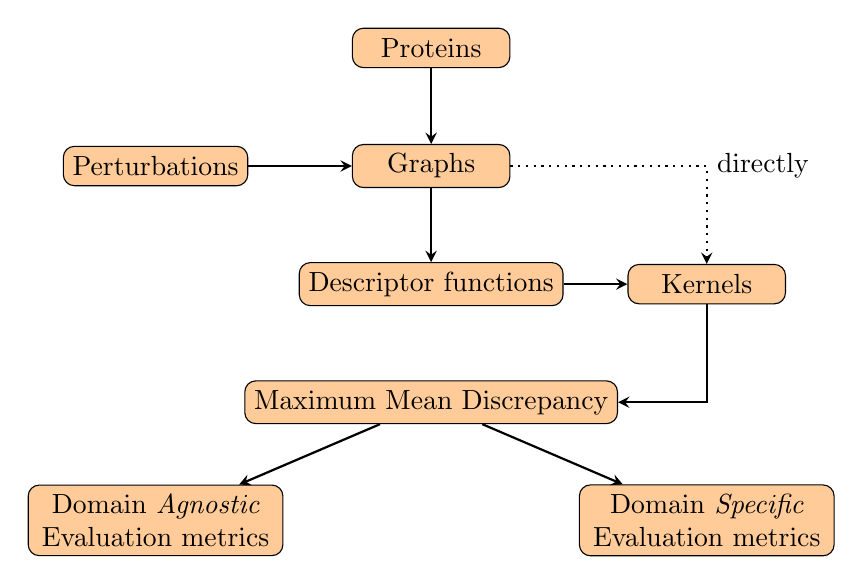
\begin{tikzpicture}[align=center, node distance=1.5cm, align=center]
      \node (proteins) [orangebox] {Proteins};
      \node (graphs) [orangebox, below of=proteins] {Graphs};
      \node (descriptors) [orangebox, below of=graphs, align=left] {Descriptor functions};
      \node (perturbations) [orangebox, left of=graphs, xshift=-2cm] {Perturbations};
      \node (kernels) [orangebox, right of=descriptors, xshift=2cm] {Kernels};

      \node (mmd) [orangebox, below of=descriptors] {Maximum Mean Discrepancy};

      \coordinate[below of=mmd] (c);
      \node (agnostic) [orangebox, left of=c, text width=3cm, xshift=-2cm] {Domain \textit{Agnostic} Evaluation metrics};
      \node (specific) [orangebox, right of=c, text width=3cm, xshift=2cm] {Domain \textit{Specific}  Evaluation metrics};

      \draw [arrow] (proteins) -- (graphs);
      \draw [arrow] (graphs) -- (descriptors);
      \draw [arrow,dotted] (graphs) -| node[anchor=west] {directly} (kernels);
      \draw [arrow] (descriptors) -- (kernels);
      \draw [arrow] (kernels) |- (mmd);

      \draw [arrow] (perturbations) -- (graphs);

      \draw [arrow] (mmd) -- (agnostic);
      \draw [arrow] (mmd) -- (specific);

      % \draw [arrow] (mmd) -- (eval);
    \end{tikzpicture}
    \caption{Overview of the library}
    \label{fig:overview}
  \end{figure}
\end{frame}

\begin{frame}[fragile]{Protein source datasets}
  \begin{itemize}
  \item Start with human proteome from AlphaFold (23390 samples,
    \href{https://ftp.ebi.ac.uk/pub/databases/alphafold/latest/UP000005640_9606_HUMAN_v2.tar}{source})
  \item Expand to other experimentally datasets \& add cleaning handlers
  \end{itemize}
\end{frame}

\begin{frame}[fragile]{Graph extraction from pdb file}
  \minipage{0.7\textwidth}
  Granularity:
  \begin{itemize}
  \item CA-atom (1 point per amino acid)
  \item all atoms (loop through each residue to get atom coordinates)
  \item CB, C, O, ... see \href{https://biopython.org/docs/1.75/api/Bio.PDB.Residue.html}{\texttt{Bio.PDB.Residue}}
  \end{itemize}
  Graph extraction:
  \begin{itemize}
  \item Contact map (fully connected weighted graph).
  \item $\varepsilon$-neighborhood graph. \cite{anastasiu2016algorithms}
  \item k-nearest neighbor graph. \cite{zhao2021approximate}
  \item \textcolor{blue}{Graph of all atoms with their bond type (incl. e.g. disulfide bond)}

  \end{itemize}

  Dependencies
  \begin{itemize}
  \item only depend on \texttt{Biopython} to manipulate \texttt{.pdb} files.
  \end{itemize}
  \endminipage
  \minipage{0.3\textwidth}
  \begin{figure}[center]
    \centering
    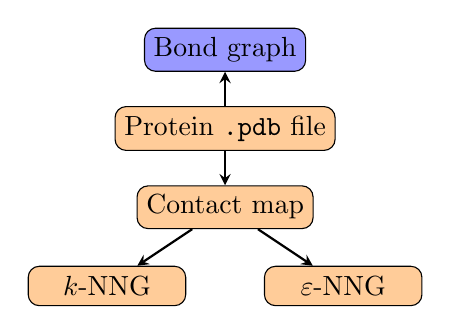
\begin{tikzpicture}[align=center, node distance=1cm, align=center]

      \node (proteins) [orangebox] {Protein \texttt{.pdb} file};
      \node (bond) [bluebox, above of=proteins] {Bond graph};
      \node (contact) [orangebox, below of=proteins] {Contact map};
      \coordinate[below of=contact] (c);
      \node (eNNG) [orangebox, right of=c, xshift=0.5cm] {$\varepsilon$-NNG};
      \node (kNNG) [orangebox, left of=c, xshift=-0.5cm] {$k$-NNG};
      \draw [arrow] (proteins) -- (contact);
      \draw [arrow] (contact) -- (eNNG);
      \draw [arrow] (contact) -- (kNNG);
      \draw [arrow] (proteins) -- (bond);
    \end{tikzpicture}
    \caption{Order of extraction of graphs from \texttt{.pdb} files.}
    \label{fig:overview}
  \end{figure}
  \endminipage

\end{frame}

\begin{frame}[fragile]{Descriptor functions \& Kernels}
  \minipage[t]{0.5\textwidth}
  \textbf{Descriptor functions} \\
  Domain agnostic graph descriptors \cite{o2021evaluation}:
  \begin{itemize}
  \item Degree distribution histogram
  \item Clustering coefficient histogram
  \item Laplacian spectrum histogram
  \end{itemize}

  Topological descriptors (using the weighted, fully connected contact map):
  \begin{itemize}
  \item Persistence diagram, converted to Betti curves, persistence image, persistence landscapes. \cite{tauzin2021giotto}
  \item Also possible to obtain vector representation from persistence diagram by applying a heat kernel to it. \cite{reininghaus2015stable}
  \end{itemize}

  Domain specific: t.b.d
  \endminipage
  \minipage[t]{0.05\textwidth}
  \hfill\vline\hfill
  \endminipage
  \minipage[t]{0.45\textwidth}
  \textbf{Kernels} \\
  Conditions for selection: p.s.d \& fast\\
  General kernels \cite{o2021evaluation}:
    \begin{itemize}
    \item RBF kernel
    \item Laplacian kernel
    \item Linear
    \item \textcolor{blue}{Neighborhood Subgraph Pairwise Distance graph kernel} \cite{costa2010fast}
    \end{itemize}
    The last can be used when dicrete edge features are employed.\\
  Domain specific: t.b.d
  \endminipage
\end{frame}

\begin{frame}[fragile]{Maximum Mean Discrepancy}
  The Maximum Mean Discrepancy (MMD) \cite{gretton2012kernel,borgwardt2006integrating} is defined as follows:
  \begin{equation*}
    \label{eq:mmd}
    \text{MMD}(X, Y) := {1\over n^2} \sum_{i,j=1}^{n}k(x_i, x_j) + {1\over m^2} \sum_{i,j=1}^{n}k(y_i, y_j) - {2\over nm} \sum_{i=1}^{n}\sum_{j=1}^{m}k(y_i, y_j)
  \end{equation*}
  where:
  \begin{itemize}
  \item  $x_i, x_j \sim \mathcal{X}$, $n$ is the number of samples from non-empty set $\mathcal{X}$;
  \item  $y_i, y_j \sim \mathcal{Y}$, $m$ is the number of samples from non-empty set $\mathcal{Y}$;
  \item $k: \mathcal{X}\times\mathcal{X}\to\mathbb{R}$ is a valid kernel.
  \end{itemize}
  MMD is a kernelized proxy of the distance between two graph distributions $G$ and $G*$ computed as $d_{\text{MMD}}(G,G^*)=MMD(f(G),f(G^*))$, where $f$ is the descriptor function of the graph. A lower $d_{\text{MMD}}(G,G^*)$ indicates a greater similarity between $G$ and $G*$.
  \textcolor{blue}{Potentially look at other metrics for GNNs. \cite{thompson2022evaluation}}
\end{frame}

\begin{frame}[fragile]{Perturbations to graphs}
  Domain agnostic \cite{o2021evaluation}:
  \begin{itemize}
  \item edge insertion
  \item edge removal
  \item edge rewiring
  \item node addition
  \end{itemize}

  Domain specific:
  \begin{itemize}
  \item t.b.d. (e.g. add edge ``disrupting'' binding pocket, how to do this?)
  \end{itemize}
\end{frame}

\begin{frame}[fragile]{Evaluation}
  Domain agnostic \cite{o2021evaluation}:
  \begin{itemize}
  \item Correlation with perturbation
  \item Correlation with graph edit distance
  \end{itemize}

  Domain specific:
  \begin{itemize}
  \item Alignment
  \item (estimated) folding energy
  \item Investigate what makes a ``good'' protein.
  \end{itemize}
\end{frame}

\begin{frame}[fragile]{Workflows enabled by the package}
  \begin{figure}[center]
    \centering
    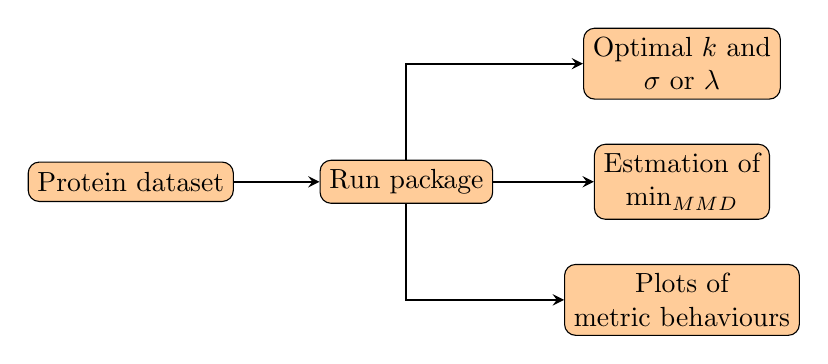
\begin{tikzpicture}[align=center, node distance=1.5cm, align=center]

      \node (dataset) [orangebox] {Protein dataset};
      \node (run) [orangebox, right of=dataset, xshift=2cm] {Run package};
      \node (min) [orangebox, right of=run, xshift=2cm] {Estmation of\\ $\min_{MMD}$};
      \node (optimal) [orangebox, above of=min] {Optimal $k$ and \\ $\sigma$ or $\lambda$};
      \node (plots) [orangebox, below of=min] {Plots of  \\metric behaviours};
      \draw [arrow] (dataset) -- (run);
      \draw [arrow] (run) |- (optimal);
      \draw [arrow] (run) -- (min);
      \draw [arrow] (run) |- (plots);
    \end{tikzpicture}
    \caption{Workflows enabled by the package.}
    \label{fig:overview}
  \end{figure}

\end{frame}

\begin{frame}[fragile]{Plots to understand the behaviour of MMD}
  \begin{itemize}
  \item Distribution of $\min_{MMD}$ for different random test/train splits.
  \item Correlation perturbation with MMD values with different parameters
  \item MMD vs. parameter
  \end{itemize}
\end{frame}

\begin{frame}[allowframebreaks]{References}

  \bibliography{../../thesis/refs.bib}
  \bibliographystyle{abbrv}

\end{frame}


\end{document}
